\documentclass[twoside]{book}

% Packages required by doxygen
\usepackage{fixltx2e}
\usepackage{calc}
\usepackage{doxygen}
\usepackage[export]{adjustbox} % also loads graphicx
\usepackage{graphicx}
\usepackage[utf8]{inputenc}
\usepackage{makeidx}
\usepackage{multicol}
\usepackage{multirow}
\PassOptionsToPackage{warn}{textcomp}
\usepackage{textcomp}
\usepackage[nointegrals]{wasysym}
\usepackage[table]{xcolor}

% Font selection
\usepackage[T1]{fontenc}
\usepackage[scaled=.90]{helvet}
\usepackage{courier}
\usepackage{amssymb}
\usepackage{sectsty}
\renewcommand{\familydefault}{\sfdefault}
\allsectionsfont{%
  \fontseries{bc}\selectfont%
  \color{darkgray}%
}
\renewcommand{\DoxyLabelFont}{%
  \fontseries{bc}\selectfont%
  \color{darkgray}%
}
\newcommand{\+}{\discretionary{\mbox{\scriptsize$\hookleftarrow$}}{}{}}

% Page & text layout
\usepackage{geometry}
\geometry{%
  a4paper,%
  top=2.5cm,%
  bottom=2.5cm,%
  left=2.5cm,%
  right=2.5cm%
}
\tolerance=750
\hfuzz=15pt
\hbadness=750
\setlength{\emergencystretch}{15pt}
\setlength{\parindent}{0cm}
\setlength{\parskip}{3ex plus 2ex minus 2ex}
\makeatletter
\renewcommand{\paragraph}{%
  \@startsection{paragraph}{4}{0ex}{-1.0ex}{1.0ex}{%
    \normalfont\normalsize\bfseries\SS@parafont%
  }%
}
\renewcommand{\subparagraph}{%
  \@startsection{subparagraph}{5}{0ex}{-1.0ex}{1.0ex}{%
    \normalfont\normalsize\bfseries\SS@subparafont%
  }%
}
\makeatother

% Headers & footers
\usepackage{fancyhdr}
\pagestyle{fancyplain}
\fancyhead[LE]{\fancyplain{}{\bfseries\thepage}}
\fancyhead[CE]{\fancyplain{}{}}
\fancyhead[RE]{\fancyplain{}{\bfseries\leftmark}}
\fancyhead[LO]{\fancyplain{}{\bfseries\rightmark}}
\fancyhead[CO]{\fancyplain{}{}}
\fancyhead[RO]{\fancyplain{}{\bfseries\thepage}}
\fancyfoot[LE]{\fancyplain{}{}}
\fancyfoot[CE]{\fancyplain{}{}}
\fancyfoot[RE]{\fancyplain{}{\bfseries\scriptsize Generated by Doxygen }}
\fancyfoot[LO]{\fancyplain{}{\bfseries\scriptsize Generated by Doxygen }}
\fancyfoot[CO]{\fancyplain{}{}}
\fancyfoot[RO]{\fancyplain{}{}}
\renewcommand{\footrulewidth}{0.4pt}
\renewcommand{\chaptermark}[1]{%
  \markboth{#1}{}%
}
\renewcommand{\sectionmark}[1]{%
  \markright{\thesection\ #1}%
}

% Indices & bibliography
\usepackage{natbib}
\usepackage[titles]{tocloft}
\setcounter{tocdepth}{3}
\setcounter{secnumdepth}{5}
\makeindex

% Hyperlinks (required, but should be loaded last)
\usepackage{ifpdf}
\ifpdf
  \usepackage[pdftex,pagebackref=true]{hyperref}
\else
  \usepackage[ps2pdf,pagebackref=true]{hyperref}
\fi
\hypersetup{%
  colorlinks=true,%
  linkcolor=blue,%
  citecolor=blue,%
  unicode%
}

% Custom commands
\newcommand{\clearemptydoublepage}{%
  \newpage{\pagestyle{empty}\cleardoublepage}%
}

\usepackage{caption}
\captionsetup{labelsep=space,justification=centering,font={bf},singlelinecheck=off,skip=4pt,position=top}

%===== C O N T E N T S =====

\begin{document}

% Titlepage & ToC
\hypersetup{pageanchor=false,
             bookmarksnumbered=true,
             pdfencoding=unicode
            }
\pagenumbering{alph}
\begin{titlepage}
\vspace*{7cm}
\begin{center}%
{\Large Docker Proxy }\\
\vspace*{1cm}
{\large Generated by Doxygen 1.8.14}\\
\end{center}
\end{titlepage}
\clearemptydoublepage
\pagenumbering{roman}
\tableofcontents
\clearemptydoublepage
\pagenumbering{arabic}
\hypersetup{pageanchor=true}

%--- Begin generated contents ---
\chapter{Synopsis}
\label{md__r_e_a_d_m_e}
\Hypertarget{md__r_e_a_d_m_e}
docker proxy 
\chapter{Hierarchical Index}
\section{Class Hierarchy}
This inheritance list is sorted roughly, but not completely, alphabetically\+:\begin{DoxyCompactList}
\item Exception\begin{DoxyCompactList}
\item \contentsline{section}{docker-\/proxy.my\+\_\+proxy.\+Invalid\+Usage}{\pageref{classdocker-proxy_1_1my__proxy_1_1_invalid_usage}}{}
\end{DoxyCompactList}
\item Model\begin{DoxyCompactList}
\item \contentsline{section}{docker-\/proxy.models.\+Container\+Names}{\pageref{classdocker-proxy_1_1models_1_1_container_names}}{}
\item \contentsline{section}{docker-\/proxy.my\+\_\+proxy.\+Container\+Names}{\pageref{classdocker-proxy_1_1my__proxy_1_1_container_names}}{}
\item \contentsline{section}{docker-\/proxy.my\+\_\+proxy.\+Mount\+Points}{\pageref{classdocker-proxy_1_1my__proxy_1_1_mount_points}}{}
\end{DoxyCompactList}
\item Test\+Case\begin{DoxyCompactList}
\item \contentsline{section}{docker-\/proxy.unit\+\_\+tests.\+Md5\+Test}{\pageref{classdocker-proxy_1_1unit__tests_1_1_md5_test}}{}
\end{DoxyCompactList}
\end{DoxyCompactList}

\chapter{Class Index}
\section{Class List}
Here are the classes, structs, unions and interfaces with brief descriptions\+:\begin{DoxyCompactList}
\item\contentsline{section}{\hyperlink{classdocker-proxy_1_1models_1_1_container_names}{docker-\/proxy.\+models.\+Container\+Names} }{\pageref{classdocker-proxy_1_1models_1_1_container_names}}{}
\item\contentsline{section}{\hyperlink{classdocker-proxy_1_1my__proxy_1_1_container_names}{docker-\/proxy.\+my\+\_\+proxy.\+Container\+Names} }{\pageref{classdocker-proxy_1_1my__proxy_1_1_container_names}}{}
\item\contentsline{section}{\hyperlink{classdocker-proxy_1_1my__proxy_1_1_invalid_usage}{docker-\/proxy.\+my\+\_\+proxy.\+Invalid\+Usage} }{\pageref{classdocker-proxy_1_1my__proxy_1_1_invalid_usage}}{}
\item\contentsline{section}{\hyperlink{classdocker-proxy_1_1unit__tests_1_1_md5_test}{docker-\/proxy.\+unit\+\_\+tests.\+Md5\+Test} }{\pageref{classdocker-proxy_1_1unit__tests_1_1_md5_test}}{}
\item\contentsline{section}{\hyperlink{classdocker-proxy_1_1my__proxy_1_1_mount_points}{docker-\/proxy.\+my\+\_\+proxy.\+Mount\+Points} }{\pageref{classdocker-proxy_1_1my__proxy_1_1_mount_points}}{}
\end{DoxyCompactList}

\chapter{Class Documentation}
\hypertarget{classdocker-proxy_1_1my__proxy_1_1_invalid_usage}{}\section{docker-\/proxy.my\+\_\+proxy.\+Invalid\+Usage Class Reference}
\label{classdocker-proxy_1_1my__proxy_1_1_invalid_usage}\index{docker-\/proxy.\+my\+\_\+proxy.\+Invalid\+Usage@{docker-\/proxy.\+my\+\_\+proxy.\+Invalid\+Usage}}
Inheritance diagram for docker-\/proxy.my\+\_\+proxy.\+Invalid\+Usage\+:\begin{figure}[H]
\begin{center}
\leavevmode
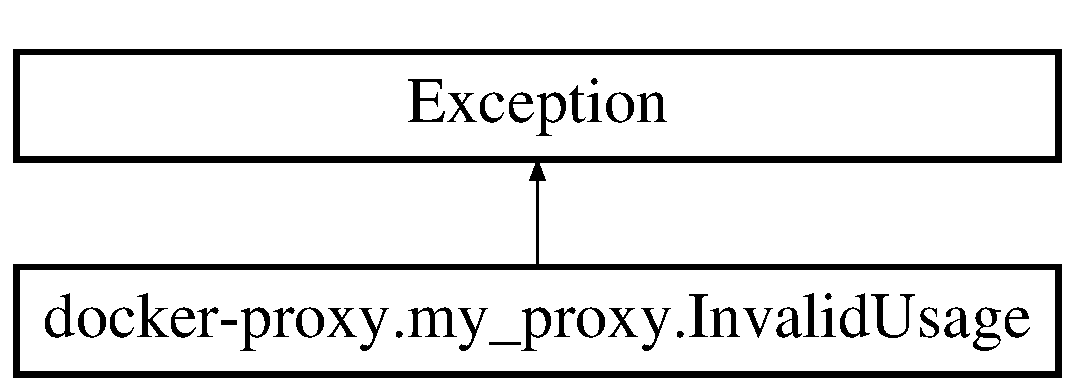
\includegraphics[height=2.000000cm]{classdocker-proxy_1_1my__proxy_1_1_invalid_usage}
\end{center}
\end{figure}
\subsection*{Public Member Functions}
\begin{DoxyCompactItemize}
\item 
\mbox{\Hypertarget{classdocker-proxy_1_1my__proxy_1_1_invalid_usage_aa785dfd5e9946eb87e2a94d4544bc656}\label{classdocker-proxy_1_1my__proxy_1_1_invalid_usage_aa785dfd5e9946eb87e2a94d4544bc656}} 
def {\bfseries \+\_\+\+\_\+init\+\_\+\+\_\+} (self, message, status\+\_\+code=None, payload=None)
\item 
\mbox{\Hypertarget{classdocker-proxy_1_1my__proxy_1_1_invalid_usage_a50b7849f7141fc1455ace3691a9417a7}\label{classdocker-proxy_1_1my__proxy_1_1_invalid_usage_a50b7849f7141fc1455ace3691a9417a7}} 
def {\bfseries to\+\_\+dict} (self)
\end{DoxyCompactItemize}
\subsection*{Public Attributes}
\begin{DoxyCompactItemize}
\item 
\mbox{\Hypertarget{classdocker-proxy_1_1my__proxy_1_1_invalid_usage_aa61d504376bb9479db82cb7d97c70011}\label{classdocker-proxy_1_1my__proxy_1_1_invalid_usage_aa61d504376bb9479db82cb7d97c70011}} 
{\bfseries message}
\item 
\mbox{\Hypertarget{classdocker-proxy_1_1my__proxy_1_1_invalid_usage_a6503499a33bc2de008fb69c03f453eec}\label{classdocker-proxy_1_1my__proxy_1_1_invalid_usage_a6503499a33bc2de008fb69c03f453eec}} 
{\bfseries status\+\_\+code}
\item 
\mbox{\Hypertarget{classdocker-proxy_1_1my__proxy_1_1_invalid_usage_a658b9343c56fde3e1753fe8ad1e1a158}\label{classdocker-proxy_1_1my__proxy_1_1_invalid_usage_a658b9343c56fde3e1753fe8ad1e1a158}} 
{\bfseries payload}
\end{DoxyCompactItemize}
\subsection*{Static Public Attributes}
\begin{DoxyCompactItemize}
\item 
\mbox{\Hypertarget{classdocker-proxy_1_1my__proxy_1_1_invalid_usage_aa06f3c7722ee51c93e799a0e57f67a32}\label{classdocker-proxy_1_1my__proxy_1_1_invalid_usage_aa06f3c7722ee51c93e799a0e57f67a32}} 
int {\bfseries status\+\_\+code} = 400
\end{DoxyCompactItemize}


\subsection{Detailed Description}
\begin{DoxyVerb}class to return specific return type codes
\end{DoxyVerb}
 

The documentation for this class was generated from the following file\+:\begin{DoxyCompactItemize}
\item 
my\+\_\+proxy.\+py\end{DoxyCompactItemize}

\hypertarget{classdocker-proxy_1_1unit__tests_1_1_md5_test}{}\section{docker-\/proxy.unit\+\_\+tests.\+Md5\+Test Class Reference}
\label{classdocker-proxy_1_1unit__tests_1_1_md5_test}\index{docker-\/proxy.\+unit\+\_\+tests.\+Md5\+Test@{docker-\/proxy.\+unit\+\_\+tests.\+Md5\+Test}}
Inheritance diagram for docker-\/proxy.unit\+\_\+tests.\+Md5\+Test\+:\begin{figure}[H]
\begin{center}
\leavevmode
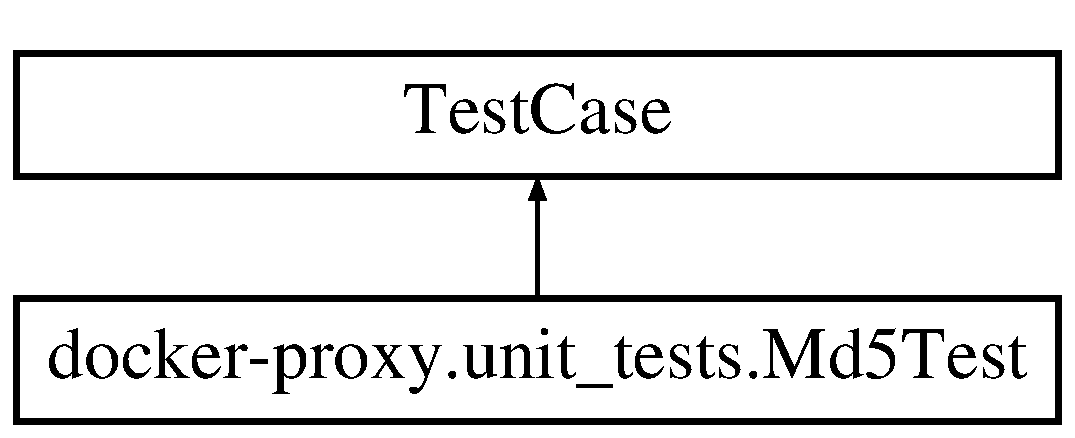
\includegraphics[height=2.000000cm]{classdocker-proxy_1_1unit__tests_1_1_md5_test}
\end{center}
\end{figure}
\subsection*{Public Member Functions}
\begin{DoxyCompactItemize}
\item 
def \mbox{\hyperlink{classdocker-proxy_1_1unit__tests_1_1_md5_test_a964cee9ecd446be83cdd9f50ff401203}{test\+\_\+is\+\_\+there\+\_\+config}} (self)
\item 
def \mbox{\hyperlink{classdocker-proxy_1_1unit__tests_1_1_md5_test_ac200f662c944e9c1f857de062fa6bd85}{test\+\_\+random\+\_\+port\+\_\+generator\+\_\+not\+\_\+restricred}} (self)
\item 
def \mbox{\hyperlink{classdocker-proxy_1_1unit__tests_1_1_md5_test_acc4c5dfd97e4925662798cd78a992772}{test\+\_\+random\+\_\+port\+\_\+generator\+\_\+is\+\_\+int}} (self)
\item 
def \mbox{\hyperlink{classdocker-proxy_1_1unit__tests_1_1_md5_test_a7a31a78746cfbad0c3d3a740f8ab50fd}{test\+\_\+random\+\_\+volume\+\_\+is\+\_\+string}} (self)
\end{DoxyCompactItemize}


\subsection{Member Function Documentation}
\mbox{\Hypertarget{classdocker-proxy_1_1unit__tests_1_1_md5_test_a964cee9ecd446be83cdd9f50ff401203}\label{classdocker-proxy_1_1unit__tests_1_1_md5_test_a964cee9ecd446be83cdd9f50ff401203}} 
\index{docker-\/proxy\+::unit\+\_\+tests\+::\+Md5\+Test@{docker-\/proxy\+::unit\+\_\+tests\+::\+Md5\+Test}!test\+\_\+is\+\_\+there\+\_\+config@{test\+\_\+is\+\_\+there\+\_\+config}}
\index{test\+\_\+is\+\_\+there\+\_\+config@{test\+\_\+is\+\_\+there\+\_\+config}!docker-\/proxy\+::unit\+\_\+tests\+::\+Md5\+Test@{docker-\/proxy\+::unit\+\_\+tests\+::\+Md5\+Test}}
\subsubsection{\texorpdfstring{test\+\_\+is\+\_\+there\+\_\+config()}{test\_is\_there\_config()}}
{\footnotesize\ttfamily def docker-\/proxy.\+unit\+\_\+tests.\+Md5\+Test.\+test\+\_\+is\+\_\+there\+\_\+config (\begin{DoxyParamCaption}\item[{}]{self }\end{DoxyParamCaption})}

\begin{DoxyVerb}Test if there is config file
:return:
\end{DoxyVerb}
 \mbox{\Hypertarget{classdocker-proxy_1_1unit__tests_1_1_md5_test_acc4c5dfd97e4925662798cd78a992772}\label{classdocker-proxy_1_1unit__tests_1_1_md5_test_acc4c5dfd97e4925662798cd78a992772}} 
\index{docker-\/proxy\+::unit\+\_\+tests\+::\+Md5\+Test@{docker-\/proxy\+::unit\+\_\+tests\+::\+Md5\+Test}!test\+\_\+random\+\_\+port\+\_\+generator\+\_\+is\+\_\+int@{test\+\_\+random\+\_\+port\+\_\+generator\+\_\+is\+\_\+int}}
\index{test\+\_\+random\+\_\+port\+\_\+generator\+\_\+is\+\_\+int@{test\+\_\+random\+\_\+port\+\_\+generator\+\_\+is\+\_\+int}!docker-\/proxy\+::unit\+\_\+tests\+::\+Md5\+Test@{docker-\/proxy\+::unit\+\_\+tests\+::\+Md5\+Test}}
\subsubsection{\texorpdfstring{test\+\_\+random\+\_\+port\+\_\+generator\+\_\+is\+\_\+int()}{test\_random\_port\_generator\_is\_int()}}
{\footnotesize\ttfamily def docker-\/proxy.\+unit\+\_\+tests.\+Md5\+Test.\+test\+\_\+random\+\_\+port\+\_\+generator\+\_\+is\+\_\+int (\begin{DoxyParamCaption}\item[{}]{self }\end{DoxyParamCaption})}

\begin{DoxyVerb}test if random port is generating an int
:return:
\end{DoxyVerb}
 \mbox{\Hypertarget{classdocker-proxy_1_1unit__tests_1_1_md5_test_ac200f662c944e9c1f857de062fa6bd85}\label{classdocker-proxy_1_1unit__tests_1_1_md5_test_ac200f662c944e9c1f857de062fa6bd85}} 
\index{docker-\/proxy\+::unit\+\_\+tests\+::\+Md5\+Test@{docker-\/proxy\+::unit\+\_\+tests\+::\+Md5\+Test}!test\+\_\+random\+\_\+port\+\_\+generator\+\_\+not\+\_\+restricred@{test\+\_\+random\+\_\+port\+\_\+generator\+\_\+not\+\_\+restricred}}
\index{test\+\_\+random\+\_\+port\+\_\+generator\+\_\+not\+\_\+restricred@{test\+\_\+random\+\_\+port\+\_\+generator\+\_\+not\+\_\+restricred}!docker-\/proxy\+::unit\+\_\+tests\+::\+Md5\+Test@{docker-\/proxy\+::unit\+\_\+tests\+::\+Md5\+Test}}
\subsubsection{\texorpdfstring{test\+\_\+random\+\_\+port\+\_\+generator\+\_\+not\+\_\+restricred()}{test\_random\_port\_generator\_not\_restricred()}}
{\footnotesize\ttfamily def docker-\/proxy.\+unit\+\_\+tests.\+Md5\+Test.\+test\+\_\+random\+\_\+port\+\_\+generator\+\_\+not\+\_\+restricred (\begin{DoxyParamCaption}\item[{}]{self }\end{DoxyParamCaption})}

\begin{DoxyVerb}Test if random generated port is not in restricted list
:return:
\end{DoxyVerb}
 \mbox{\Hypertarget{classdocker-proxy_1_1unit__tests_1_1_md5_test_a7a31a78746cfbad0c3d3a740f8ab50fd}\label{classdocker-proxy_1_1unit__tests_1_1_md5_test_a7a31a78746cfbad0c3d3a740f8ab50fd}} 
\index{docker-\/proxy\+::unit\+\_\+tests\+::\+Md5\+Test@{docker-\/proxy\+::unit\+\_\+tests\+::\+Md5\+Test}!test\+\_\+random\+\_\+volume\+\_\+is\+\_\+string@{test\+\_\+random\+\_\+volume\+\_\+is\+\_\+string}}
\index{test\+\_\+random\+\_\+volume\+\_\+is\+\_\+string@{test\+\_\+random\+\_\+volume\+\_\+is\+\_\+string}!docker-\/proxy\+::unit\+\_\+tests\+::\+Md5\+Test@{docker-\/proxy\+::unit\+\_\+tests\+::\+Md5\+Test}}
\subsubsection{\texorpdfstring{test\+\_\+random\+\_\+volume\+\_\+is\+\_\+string()}{test\_random\_volume\_is\_string()}}
{\footnotesize\ttfamily def docker-\/proxy.\+unit\+\_\+tests.\+Md5\+Test.\+test\+\_\+random\+\_\+volume\+\_\+is\+\_\+string (\begin{DoxyParamCaption}\item[{}]{self }\end{DoxyParamCaption})}

\begin{DoxyVerb}test of random volume name is str
:return:
\end{DoxyVerb}
 

The documentation for this class was generated from the following file\+:\begin{DoxyCompactItemize}
\item 
unit\+\_\+tests.\+py\end{DoxyCompactItemize}

%--- End generated contents ---

% Index
\backmatter
\newpage
\phantomsection
\clearemptydoublepage
\addcontentsline{toc}{chapter}{Index}
\printindex

\end{document}
